\documentclass[border=5pt]{standalone}
\usepackage{amsmath}
\usepackage{tikz}
\usetikzlibrary{shapes}

\begin{document}

\begin{minipage}{15.5cm}
\begin{figure}[tb]
    \centering
\begin{tikzpicture}
\node[anchor=south west,inner sep=0] at (-3.31,-2.12) {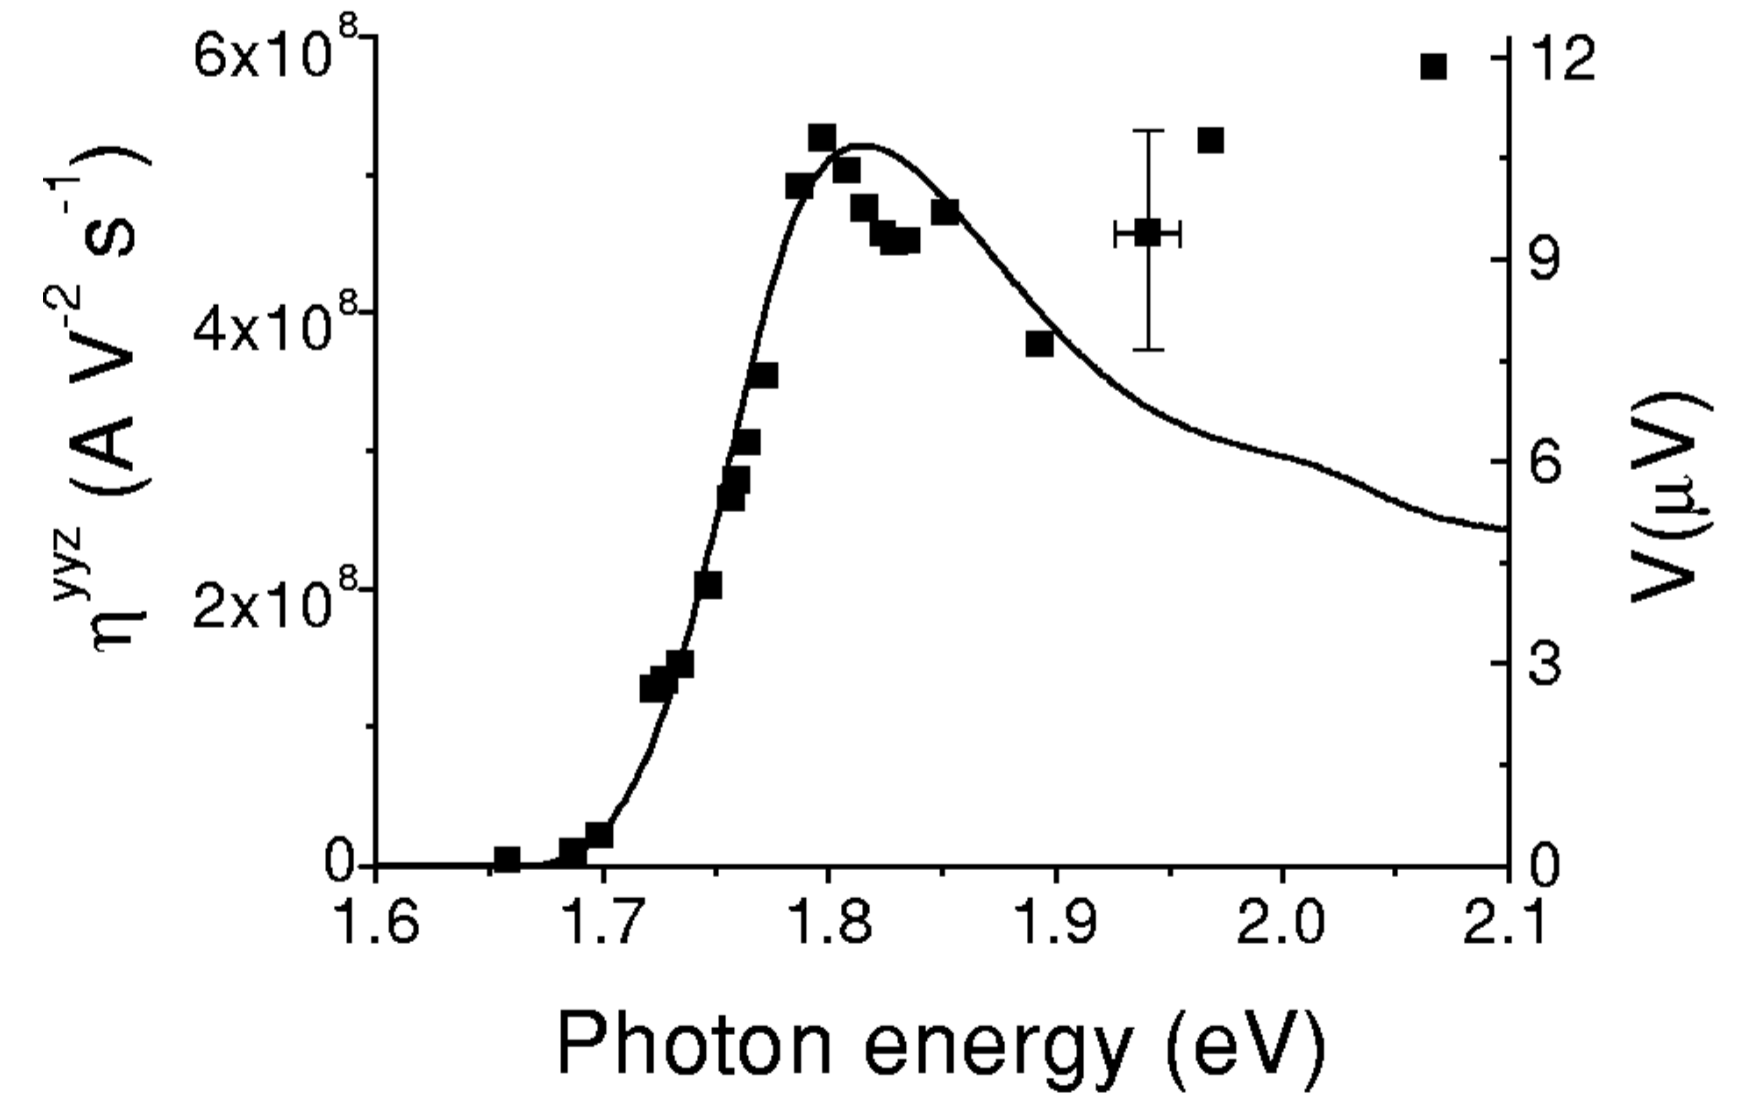
\includegraphics[width=15.35cm]{lamanAPL99-Fig3.png}};

% border:
    % border height: 
    \def \ymax {7.12}
    % border lenght
    \def \xmax {10.0}
    \draw[red, thick] (0,0) -- (\xmax,0) -- (\xmax,\ymax) -- (0,\ymax) -- cycle;

% subdivitions:
    % x and y divitions:
    \def \xdiv {10}
    \def \ydiv {12}
    \def \yDiv {\ydiv*10}

% grid:
    \def \ythickdiv {\ymax/\ydiv}
    \def \xthickdiv {\xmax/\xdiv}
    \def \ytindiv {\ydiv*10}
    % tin grid:
    \def \ytindiv {\ythickdiv*0.1}
    \foreach \i in {1,...,120}{\draw[green] (0,\ytindiv*\i) -- (\xmax,\ytindiv*\i);}
    \def \xtindiv {\xthickdiv*0.1}
    \foreach \i in {1,...,100}{\draw[green] (\xtindiv*\i,0) -- (\xtindiv*\i,\ymax);}
    % thick grid:
    \foreach \i in {1,...,\ydiv}{\draw[red, thick] (0,\ythickdiv*\i) -- (\xmax,\ythickdiv*\i);}
    \foreach \i in {1,...,10}{\draw[red, thick] (\xthickdiv*\i,0) -- (\xthickdiv*\i,\ymax);}

% experimental points:

% \node at (0,-1) {\pgfuseplotmark{*}};

\node [blue] at (1.16,0.089) {\pgfuseplotmark{*}};
\node [blue] at (1.74,0.119) {\pgfuseplotmark{*}};
\node [blue] at (1.94,0.267) {\pgfuseplotmark{*}};
\node [blue] at (2.44,1.572) {\pgfuseplotmark{*}};
\node [blue] at (2.54,1.661) {\pgfuseplotmark{*}};
\node [blue] at (2.70,1.780) {\pgfuseplotmark{*}};
\node [blue] at (2.94,2.492) {\pgfuseplotmark{*}};
\node [blue] at (3.14,3.293) {\pgfuseplotmark{*}};
\node [blue] at (3.20,3.412) {\pgfuseplotmark{*}};
\node [blue] at (3.30,3.797) {\pgfuseplotmark{*}};
\node [blue] at (3.40,4.391) {\pgfuseplotmark{*}};
\node [blue] at (3.74,6.022) {\pgfuseplotmark{*}};
\node [blue] at (3.94,6.408) {\pgfuseplotmark{*}};
\node [blue] at (4.14,6.111) {\pgfuseplotmark{*}};
\node [blue] at (4.30,5.815) {\pgfuseplotmark{*}};
\node [blue] at (4.50,5.577) {\pgfuseplotmark{*}};
\node [blue] at (4.60,5.518) {\pgfuseplotmark{*}};
\node [blue] at (4.70,5.548) {\pgfuseplotmark{*}};
\node [blue] at (5.04,5.755) {\pgfuseplotmark{*}};
\node [blue] at (5.86,4.598) {\pgfuseplotmark{*}};
\node [blue] at (6.80,5.577) {\pgfuseplotmark{*}};
\node [blue] at (7.34,6.408) {\pgfuseplotmark{*}};
\node [blue] at (9.34,7.031) {\pgfuseplotmark{*}};
\end{tikzpicture}
\caption{Fig (3) from  APL \textbf{75}, 17 2581--2583 (1999). Original caption:
Calculated spectral dependence of  $\eta^{yyz}$ in CdSe. The data represent the
spectral dependence of current injection using a 130 fs optical paramet- ric
amplifier; the vertical scales have been chosen to yield a common peak
amplitude.}
\label{fig:experimental_data}
\end{figure}
Experimental data extracted:
\begin{center}
\begin{tabular}{ccc}
Point &   Photon energy (Ev) &  $V$ ($\mu$V)    \\    
01    &   1.658              &  0.15 \\
02    &   1.687              &  0.20 \\
03    &   1.697              &  0.45 \\
04    &   1.722              &  2.65 \\
05    &   1.727              &  2.80 \\
06    &   1.735              &  3.00 \\
07    &   1.747              &  4.20 \\
08    &   1.757              &  5.55 \\
09    &   1.760              &  5.75 \\
10    &   1.765              &  6.40 \\
11    &   1.770              &  7.40 \\
12    &   1.787              & 10.15 \\
13    &   1.797              & 10.80 \\
14    &   1.807              & 10.30 \\
15    &   1.815              &  9.80 \\
16    &   1.825              &  9.40 \\
17    &   1.830              &  9.30 \\
18    &   1.835              &  9.35 \\
19    &   1.852              &  9.70 \\
20    &   1.893              &  7.75 \\
21    &   1.940              &  9.40 \\
22    &   1.967              &  10.8 \\
23    &   2.067              & 11.85 \\

\end{tabular}
\end{center}

\end{minipage}


\end{document}

